\documentclass[a4paper]{article}
\usepackage{cmap}
\usepackage{mathtext}
\usepackage{amssymb}
\usepackage{amsmath}
\usepackage[russian]{babel}
\usepackage{indentfirst}
\usepackage[pdftex]{graphicx}
\usepackage{multirow}
\usepackage{siunitx}
\usepackage[left=2cm,right=2cm,top=2cm,bottom=2cm]{geometry}
\usepackage{fancyhdr}
\pagestyle{fancy}
\newcommand{\rref}[1]{(\ref{#1})}
\newcommand{\Equip}[3]{
	
	{\bf #1:} $\Delta = \pm #2$ \si{#3}
	
}
\newcommand{\equip}[1]{
	
	{\bf #1}
	
}
\newcommand{\labname}{Вынужденные колебания в электрическом контуре.} 	% название пиши здесь
\newcommand{\labnum}{3.2.5.}										% номер вводи здесь
\fancyfoot{}
\fancyhead[RE, RO]{\thepage}
\fancyhead[LE, LO]{Лабораторная работа \labnum \space \labname}
\title{Лабораторная работа \labnum \space \labname}
\author{Иван Сладков}
\begin{document}
\maketitle
\thispagestyle{empty}
\section{Аннотация}
В данной работе проводится исследование вынужденных колебаний и процессов их установления под воздействием внешней ЭДС, которая гармонически меняется со временем; а также расчёт добротности контура несколькими способами: через исследование резонансных кривых, процессов установления и затухания колебаний; а также теоретически.
\section{Теоретические сведения}

Колебания в RLC-контуре представляют собой суперпозицию двух синусоид:
\begin{equation}
	I= B e^{-\gamma t} \sin (\omega t - \Theta)+ \frac{\mathcal{E}_0 \Omega}{L \rho_0} \sin (\Omega t - \psi),
	\label{law}
\end{equation}
При подключении контура к синусоидальной ЭДС собственные колебания с частотой $\omega$ со временем затухают. Однако при совпадении внешней частоты $ \Omega $ и собственной $ \omega $ возникает резонанс, при котором амплитуда вынужденных колебаний достигает максимального значения. Зависимость амплитуды установившихся колебаний от внешней частоты называется резонансной кривой.

Для достоверного исследования резонансной кривой необходимо, чтобы импеданс исследуемого участка цепи не зависел от импеданса источника питания даже на резонансе. С этой целью в работе используется параллельный колебательный контур (рис. \ref{fig:scheme})
\begin{figure}
	\centering
	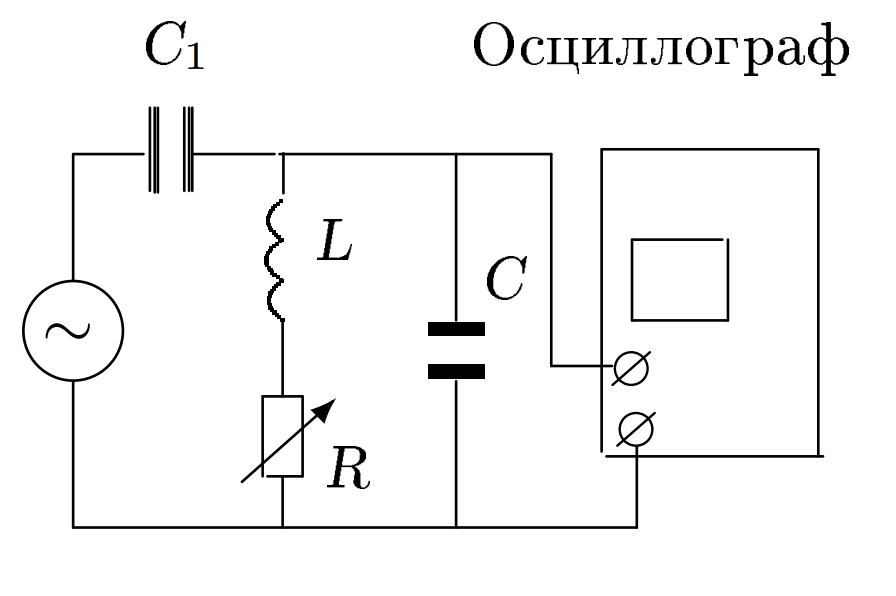
\includegraphics[width=0.8\linewidth]{Screenshot_1}
	\caption{Схема параллельного колебательного контура}
	\label{fig:scheme}
\end{figure}
Зависимость напряжения для конденсатора С $ U(\Omega) $ будет практически такой же, как в последовательном контуре при условии, что импедансы возбуждающей и измеряющей цепей существенно больше, чем импеданс исследуемой цепи. Таким образом,
\begin{equation}
	\frac{1}{\omega C_1}\gg \frac{L}{R C}, \; \; R_O \gg \frac{L}{R C},
\end{equation}
где $ R_O \simeq 1$ \si{\mega \ohm} -- сопротивление на входе осциллографа.

По ширине резонансной кривой определяется добротность контура из формулы:
\begin{equation}
	Q = \frac{\omega_0}{2 \Delta \Omega} = \frac{\nu_0}{\Delta \nu},
	\label{eq:main}
\end{equation}
где $ \omega_0 = 2 \pi \nu_0 $ -- резонансная циклическая частота.

Добротность контура также можно определить по скорости возрастания амплитуды вынужденных колебаний, а также по скорости затухания свободных при резонансном значении частоты (что немаловажно). Обоими этими способами можно воспользоваться, если подавать колебания в контур цугами, то есть отрезками синусоиды в несколько периодов. 

\subsection{Расчётные формулы}

\emph{Все формулы и расчёты приведены в системе СИ.}

Теоретическое определение резонансной частоты проводится по формуле:
\begin{equation}\label{nu}
	\nu_0 = \frac{1}{2 \pi \sqrt{L C}}
\end{equation}

Для определения добротности первым способом будем использовать формулу \rref{eq:main}, измеряя $ \Delta \Omega $ на уровне 0.7 от резонансной амплитуды.

Для определения вторым способом применим формулы:
\begin{equation}
	\Theta^\searrow = \frac{1}{n} \ln \frac{U_k}{U_{k+n}},
\end{equation}
\begin{equation}\label{key}
	\Theta^\nearrow = \frac{1}{n} \ln \frac{U_0 - U_k}{U_0 - U_{k+n}},	
\end{equation}
\begin{equation}
	Q = \frac{\pi}{\Theta}.
\end{equation}

Добротность также можно рассчитать теоретически через параметры контура по формуле:
\begin{equation}\label{teor}
	Q = \frac{1}{R } \sqrt{\frac{L}{C}}
\end{equation}

\section{Оборудование и инструментальные погрешности}
Схема установки, применяемой в эксперименте, представлена на рис. \ref{fig:set}.
\begin{figure}
	\centering
	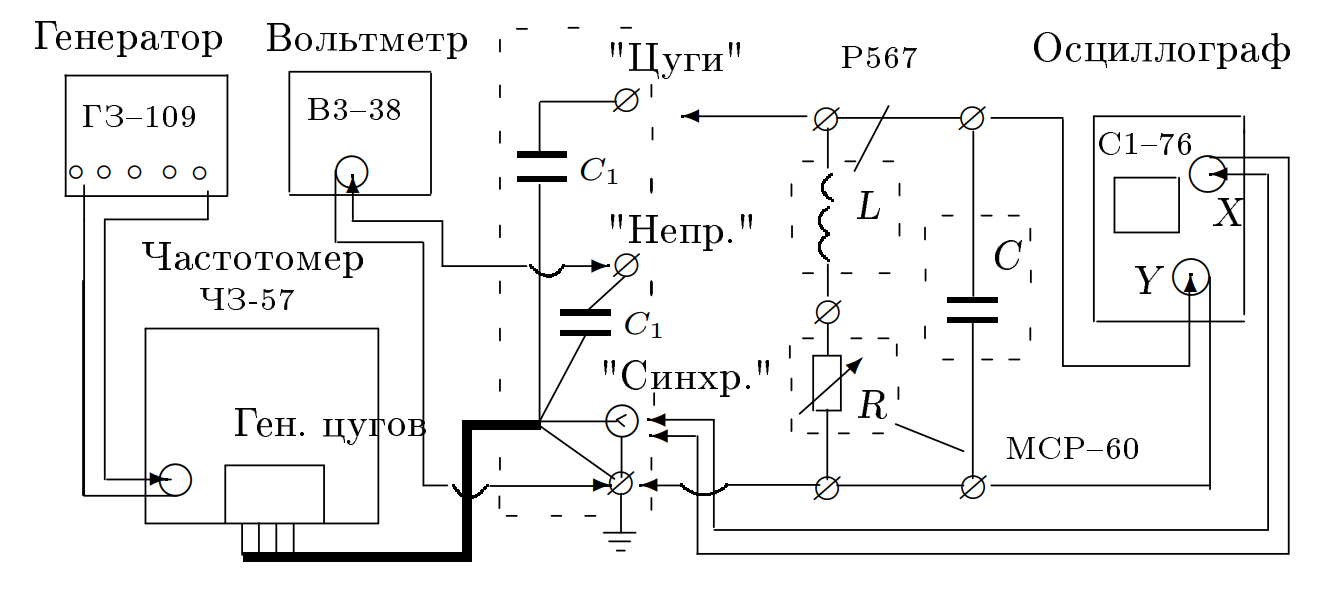
\includegraphics[width=1\linewidth]{Screenshot_2}
	\caption{Схема экспериментальной установки}
	\label{fig:set}
\end{figure}
Генератор цугов встроен в частотомер. Настройка приборов и сборка схемы проведена в соответствии с дополнительным описанием. Универсальный RLC-измеритель на схеме не показан.
\equip{Генератор звуковой частоты}
\equip{Осциллограф}
\Equip{Вольтметр}{0.1}{\volt}
\Equip{Частотомер}{1}{\hertz}
{\bf Ёмкость: }$C = 0.1$ \si{\micro \hertz}

{\bf Индуктивность: }$L = 0.1$ \si{\henry}
\equip{Магазин сопротивлений}
\equip{RLC-измеритель}

\section{Результаты измерений и обработка данных}

\subsection{Исследование резонансных кривых}

По формуле \rref{nu} рассчитаем теоретическую частоту резонанса:
\begin{equation}\label{key}
	\nu_0\approx 1592 \; Гц
\end{equation}
\begin{equation}\label{key}
	\nu_0^{эксп} \approx 1574 \; Гц.
\end{equation}
В таблице \ref{res} указаны резонансные значения напряжений.

\begin{table}[]
	\centering
	\begin{tabular}{|l|l|l|}
		\hline
		\textbf{$R$, Ом} & \textbf{$\nu_0$, Гц} & \textbf{$U_0$, В} \\ \hline
		0                & 1574                 & 8.6               \\ \hline
		100              & 1574                 & 1.9               \\ \hline
	\end{tabular}
	\caption{Резонансные значения}
	\label{res}
\end{table}

Результаты исследования резонансных кривых отображены в таблице \ref{tabb}, по которым был построен график на рис. \ref{fig:graph} в безразмерных координатах.
\begin{table}[]
	\centering
	\begin{tabular}{|l|l|l|l|}
		\hline
		\multicolumn{2}{|l|}{\textbf{R=0 Ом}}         & \multicolumn{2}{l|}{\textbf{R=100 Ом}}        \\ \hline
		\textbf{Частота, Гц} & \textbf{Напряжение, В} & \textbf{Частота, Гц} & \textbf{Напряжение, В} \\ \hline
		1495                 & 2                      & 1348                 & 0.6                    \\ \hline
		1512                 & 2.7                    & 1404                 & 0.8                    \\ \hline
		1529                 & 3.6                    & 1444                 & 1                      \\ \hline
		1546                 & 5.2                    & 1501                 & 1.4                    \\ \hline
		1559                 & 7.2                    & 1550                 & 1.8                    \\ \hline
		1575                 & 8.6                    & 1604                 & 1.8                    \\ \hline
		1593                 & 6.4                    & 1657                 & 1.5                    \\ \hline
		1603                 & 5.1                    & 1708                 & 1.2                    \\ \hline
		1627                 & 3.4                    & 1770                 & 1                      \\ \hline
		1641                 & 2.8                    & 1841                 & 0.8                    \\ \hline
		1678                 & 1.9                    & 1973                 & 0.6                    \\ \hline
	\end{tabular}
	\caption{Исходные данные для резонансных кривых}
	\label{tabb}
\end{table}
\begin{figure}[bth]
	\centering
	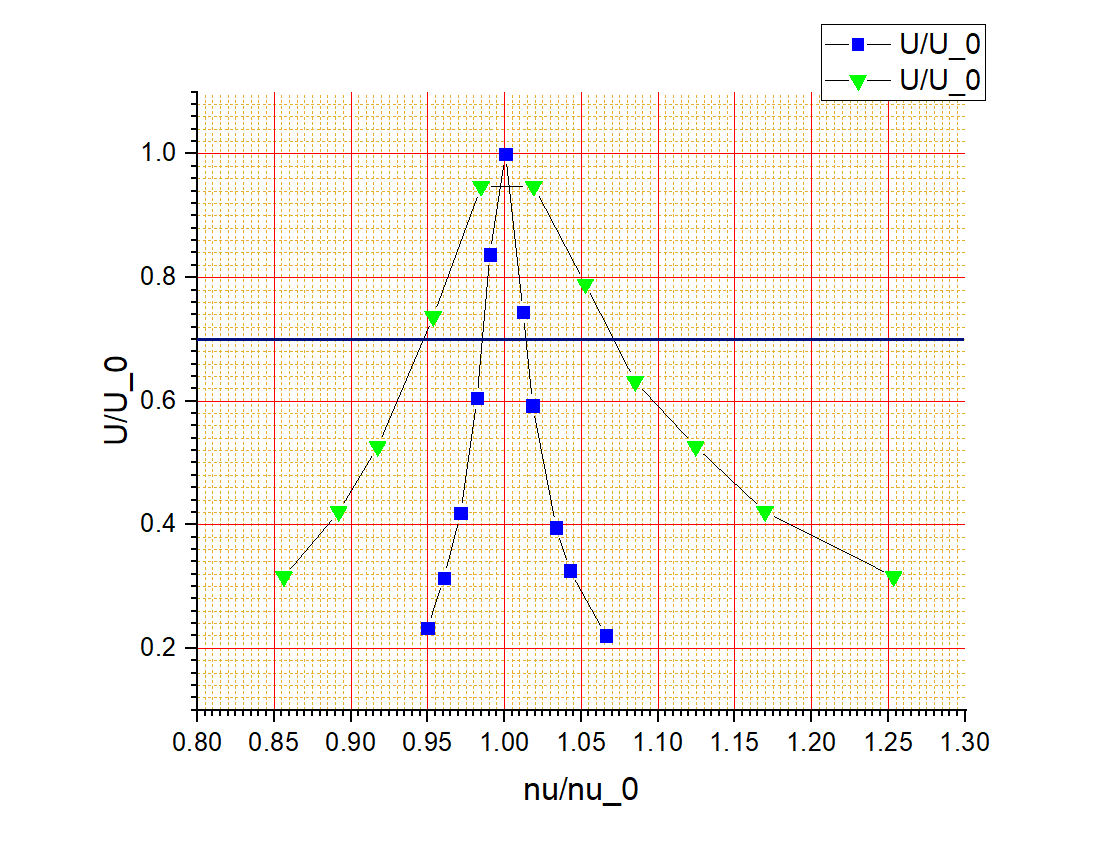
\includegraphics[width=1\linewidth]{G3}
	\caption{График резонансных кривых в безразмерных координатах $\frac{U}{U_0}(\frac{\nu}{\nu_0})$}
	\label{fig:graph}
\end{figure}
По нему на уровне $ U/U_0 = 0.7 $ определим ширину резонансной кривой и по формуле \eqref{eq:main} рассчитаем:
\begin{equation*}\label{key}
	\Delta (\frac{\nu}{\nu_0})_{R=0} = 0.03 \pm 0.007,
\end{equation*}
\begin{equation*}\label{key}
	\Delta (\frac{\nu}{\nu_0})_{R=100} = 0.12 \pm 0.03 ,
\end{equation*}
\begin{equation}\label{key}
	Q_{R=0} = \frac{1}{0.03} = 33 \pm 8,
\end{equation}
\begin{equation}\label{key}
	Q_{R=100} = \frac{1}{0.12} = 8 \pm 2,
\end{equation}

\subsection{Исследование установления и затухания колебаний}

Для каждого расчета построим таблицу.

\begin{table}[h!]
	\centering
	\begin{tabular}{|l|l|l|l|l|}
		\hline
		$\mathbf{U_k}$ & $\mathbf{U_{k+n}}$ & $\mathbf{n}$ & $\mathbf{\Theta}$ & $\mathbf{Q}$  \\ \hline
		0.2   & 0.3     & 3   & 0.0959   & 32.8 \\ \hline
		0.2   & 0.4     & 7   & 0.0990   & 31.7 \\ \hline
		0.4   & 0.5     & 7   & 0.0990   & 31.7 \\ \hline
		0.3   & 0.5     & 11  & 0.0999   & 31.5 \\ \hline
	\end{tabular}
\caption{Расчёт добротности на установлении при $R=0$}
\end{table}

\begin{table}[h!]
	\centering
	\begin{tabular}{|l|l|l|l|l|}
		\hline
		$\mathbf{U_m}$ & $\mathbf{U_{m+n}}$ & $\mathbf{n}$ & $\mathbf{\Theta}$ & $\mathbf{Q}$ \\ \hline
		0.5            & 0.2              & 10           & 0.0916            & 34.3         \\ \hline
		0.2            & 0.1              & 10           & 0.0693            & 45.3         \\ \hline
		0.3            & 0.2              & 4            & 0.101             & 31.0         \\ \hline
		0.6            & 0.4              & 5            & 0.0811            & 38.7         \\ \hline
	\end{tabular}
\caption{Расчёт добротности на затухании при $R=0$}
\end{table}

\begin{table}[h!]
	\centering
	\begin{tabular}{|l|l|l|l|l|}
		\hline
		$\mathbf{U_k}$ & $\mathbf{U_k+n}$ & $\mathbf{n}$ & $\mathbf{\Theta}$ & $\mathbf{Q}$ \\ \hline
		0.04           & 0.15             & 12           & 0.392             & 8.00         \\ \hline
		0.075          & 0.125            & 3            & 0.358             & 8.79         \\ \hline
		0.1            & 0.15             & 10           & 0.393             & 7.99         \\ \hline
	\end{tabular}
\caption{Расчёт добротности на установлении при $R=100$ Ом}
\end{table}

\begin{table}[h!]
	\centering
	\begin{tabular}{|l|l|l|l|l|}
		\hline
		$\mathbf{U_m}$ & $\mathbf{U_m+n}$ & $\mathbf{n}$ & $\mathbf{\Theta}$ & $\mathbf{Q}$ \\ \hline
		0.15           & 0.025            & 5            & 0.358             & 8.77         \\ \hline
		0.075          & 0.025            & 3            & 0.366             & 8.58         \\ \hline
		0.19           & 0.1              & 2            & 0.321             & 9.79         \\ \hline
	\end{tabular}
\caption{Расчёт добротности на затухании при $R=100$ Ом}
\end{table}

Усредним эти значения:

\begin{equation}\label{key}
	Q_{R=0} = 34 \pm 2
\end{equation}
\begin{equation}\label{key}
	Q_{R=100} = 8.6 \pm 0.2
\end{equation}

\subsection{Оценка погрешностей}
Погрешности в первом опыте оценивались в предположении, что ошибка $U/U_0$ существенно больше, чем $\nu/\nu_0$. В свою очередь, погрешность $U/U_0$ оценивалась по формуле:
\begin{equation}\label{key}
	\sigma_{\frac{U}{U_0}}=\frac{U}{U_0} \sqrt{((\sigma_U/U)^2+(\sigma_U/U_0)^2)}.
\end{equation}

Погрешности второго опыта рассчитаны в программе \emph{Origin} по формуле стандартной ошибки среднего.

\subsection{Теоретический расчёт}

Определив параметры контура, занесём их в таблицу \ref{2}.

\begin{table}[h]
	\centering
	\begin{tabular}{|l|l|l|}
		\hline
		$\mathbf{\nu}${\bf,  Гц} & $\mathbf{L}${\bf, мГн} & $\mathbf{R}${\bf, Ом} \\ \hline
		50                       & 99.975                 & 22.910                \\ \hline
		500                      & 99.953                 & 23.975                \\ \hline
		1500                     & 99.961                 & 25.554                \\ \hline
	\end{tabular}
	\caption{Параметры RLC-контура}
	\label{2}
\end{table}

На их основе рассчистаем $Q$:
\begin{equation}\label{key}
	Q_{R=0} = 39.125 \pm 0.9
\end{equation}
\begin{equation}\label{key}
	Q_{R=100}=8.15 \pm 0.19
\end{equation}
\section{Вывод}

Обобщим все полученные результаты в табл. \ref{1}. Различные методы измерения с неплохой точностью согласуются между собой. Большая погрешность измерения $Q_1$ обусловлена недостаточной точностью вольтметра. Видно, что при возрастании активного сопротивления добротность контура ухудшается, так как увеличивается количество рассеиваемой энергии.
\begin{table}[h!]
	\centering
	\begin{tabular}{|l|l||l|l|l|}
		\hline
		R      & R контура & $Q_1$      & $Q_2$         & $f(LRC)$         \\ \hline
		0      & 25.554    & $33 \pm 8$ & $34 \pm 2$    & $39.125 \pm 0.9$ \\ \hline
		100 Ом & 126.97    & $8 \pm 2$  & $8.6 \pm 0.2$ & $8.15 \pm 0.19$  \\ \hline
	\end{tabular}
	\caption{Результаты измерения добротности}
	\label{1}
\end{table}


\newpage
\begin{thebibliography}{9}
\bibitem{Siv} Сивухин Д. В. \emph{Общий курс физики. Том 3 Электричество и магнетизм}, 2004
\bibitem{Gld} Гладун А. Д. \emph{Лабораторный практикум по общей физике. Том 1 Механика}, 2004
\end{thebibliography}
\end{document}

